 % Første linje er dokumentklassen. Brug *altid* memoir!
\documentclass[a4paper,oneside,article]{memoir}

% Herunder indlæses forskellige pakker
\usepackage[utf8]{inputenc}  % Korrekt håndtering af æ, ø og å
\usepackage[T1]{fontenc}  % Korrekt håndtering af æ, ø og å
\usepackage{microtype}  % Typografisk magi! Giver bl.a. pænere orddeling
\usepackage{graphicx}  % Gør det muligt at indsætte billeder
\usepackage{amsmath}  % Giver adgang til uundværlige matematikting
\usepackage{mathtools}  % Retter ting i ams og giver ekstra muligheder
\usepackage[danish]{babel}  % Danske betegnelser og orddeling
\usepackage{lmodern}
\usepackage{alphabeta}
\usepackage{float} %Mere kontrol over billede-placering
\renewcommand{\danishhyphenmins}{22}  % Bedre dansk orddeling
\usepackage[exponent-product=\ensuremath{\cdot}]{siunitx} % Sientific notation for forskellige ting, med en regel om at den skal bruge cdot istedet for times. 
\usepackage{derivative} % Til at skrive differentialligninger 
\usepackage{xcolor} % For at få flere tekst farver 
\usepackage[colorlinks=true]{hyperref} % For at få refrences man kan trykke på, slet [] hvis man vil have kasser i stedet for farvet tekst.
\usepackage{pdfpages} % Til at indsætte andre pdf'er
\usepackage{subfig} % For at have to billeder ved siden af hinanden
\usepackage{unicode-math}

% Pænere toc indents 
\usepackage{tocloft}
\cftsetindents{section}{1em}{2em}
\cftsetindents{subsection}{4em}{0em}


% Indholdet i dit dokument starter her!
\begin{document}
\author{Mikkel Moth Billing \\ 202307989}
\title{Kvantemekanik Formelsamling}
\date{\today}
\maketitle   % Indsætter overskriften
% Table of Contents indstillinger
\setcounter{tocdepth}{2}
\setcounter{secnumdepth}{1}
\hypersetup{linkcolor=black} % Laver tableofcontents sort.  
\tableofcontents %Indsætter ToC
\hypersetup{linkcolor=red} % og så alle andre hyperrefs røde. 

%Custom Commands
%Til opgavebeskrivelser
\newcommand{\opg}[1]{\textcolor{gray}{\emph{#1}}\plainbreak{1}} 

\newcommand{\ti}[1]{\cdot 10^{#1}} % Let: gange 10^x
\newcommand{\e}[1]{\emph{e}^{#1}} % Pænere e^x
\newcommand{\vm}[2]{\begin{pmatrix} #1 \\ #2 \end{pmatrix}}
\newcommand{\mat}[1]{\begin{bmatrix} #1 \end{bmatrix}}

% Lette paranteser 
\newcommand{\br}[2][1]{%
    \ifcase#1
    \or \left( #2 \right) %1 eller ingenting
    \or \left[ #2 \right] %2
    \or \left\langle #2 \right\rangle %3
    \or \left\{ #2 \right\} %4
    \or \left| #2 \right| %5
    \fi
}
%Til at sætter bileder ind i store dokumenter
\newcommand{\bil}[1]{
\begin{figure}[H]
    \centering
    \includegraphics[width=0.75\linewidth]{Billeder/#1.png}
    \label{fig:#1}
\end{figure}
}

%Til at sætte pdf'er ind i store dokumenter (kun pdf'er på mere end 1 sider)
\newcommand{\pdf}[4]{
\includepdf[pages=#3,scale=.85,pagecommand={\subsection{#2 - \ref{ch:opg}}  \label{asc:#2}}]{pdf/#1.pdf}
\includepdf[pages=\the\numexpr 1 + #3\relax-#4, scale=.85]{pdf/#1.pdf}
}

\newcommand{\h}{\hbar}
\newcommand{\dd}{\partial}
\newcommand{\eq}[1]{\label{eq#1}\tag{#1}}
\renewcommand{\a}{\hat{a}}
\newcommand{\n}{\plainbreak{1}}
\newcommand{\ep}{\epsilon}

\newcommand{\hv}[2][]{%
    \if\relax\detokenize{#1}\relax
        |#2\rangle%
    \else
        \if\relax\detokenize{#2}\relax
            \langle #1|%
        \else
            \langle #1|#2\rangle%
        \fi
    \fi
}



% Lav ny pagestyle (kun odd fordi enkeltsidet)
\makepagestyle{Title}
\pagestyle{Title}
%\makeoddhead{Title}{\footnotesize\color{gray}{\theauthor}}{}{\textcolor{gray}{\thedate}}
\makeoddfoot{Title}{}{\footnotesize\color{gray}{\thepage{} / \thelastpage}}{}
% Også fod på siden med \maketitle
\makeoddfoot{plain}{}{\footnotesize\color{gray}{\thepage{} / \thelastpage}}{}
\newpage

%Skriv
\chapter{Schrödingers ligning}
\begin{align*}
    i\h \frac{\dd Ψ(x,t)}{\dd t} = -\frac{\h^2}{2m}\frac{\dd^2Ψ(x,t)}{\dd x^2}+V(x,t)Ψ(x,t) \eq{1.1} \\
\end{align*}

Da Bølgefunktionen kan ses som en sandsynlighed for en partikels position: 

\begin{align*}
    \int_{-\infty}^{\infty}\br[5]{Ψ(x,t)}^2dx=1 \eq{1.3}
\end{align*}

Sandsynligheden for at måle partiklen i intervallet $[a,b]$: 

\begin{align*}
    \int_{-a}^{b}\br[5]{Ψ(x,t)}^2dx
\end{align*}

For at normalisere en bølgeligning kan man bruge ligning (1.3), men hvis man normalisere bølgefunktionen 
til tiden 0, er den normaliseret til alle tider: 

\begin{align*}
    \int_{-\infty}^{\infty}\br[5]{ψ(x)}^2dx=1
\end{align*}

\n
\section{Momentum}
Middelværdi af enhver observabel operator der påvirker en partikel med en bølgefunktion, 
kan renges som: 

\begin{align*}
    \br[3]{Q(x,p)} = \int Ψ^*\br[2]{Q\br{x,-i\h\frac{\dd}{\dd x}}}Ψdx \eq{1.36} 
\end{align*}

Ehrenfest's theorem: 
\begin{align*} 
    \frac{d\br[3]{p}}{dt} = \br[3]{-\frac{\dd V}{\dd x}} \eq{1.38}
\end{align*}

\newpage
\chapter{Tidsuafhængig Schrödinger ligning}
\section{Stationær}
Hvis bølgefunktionen deles op i to dele, kan vi skrive Schrödinger ligningen på en stationær form: 
\begin{align*}
    & Ψ(x,t) = ψ(x)φ(t) \eq{2.2}\\ 
    &\Rightarrow -\frac{\h^2}{2m}\frac{\dd^2ψ(x)}{\dd x^2}+V(x)ψ(x) \eq{2.5} \\
    &\Rightarrow φ(t) = \e{-iEt/\h} \eq{2.6}
\end{align*}

(2.6) kaldes for wiggle faktoren. Hvis vi kender den tidsuafhængige bølgefunktion
kan vi regne den generelle ved at gange denne på ud fra (2.2). 

\begin{align*}
    \br[5]{Ψ(x,t)}^2 = \br[5]{ψ(x)}^2 \eq{2.8}
\end{align*}

For stationære tilstande er (\ref{eq1.36}) ikke tidsafhængig, hvilket vil sige, 
at $\br[3]{x}$ er konstant, og $\br[3]{p}=0$. 

For stationære tilstande kan den totale energi skrives som summen af den kinetiske og potentielle, 
det kaldes Hamiltonian, og skrives som en operator: 

\begin{align*}
    \hat{H} &= -\frac{\h^2}{2m}\frac{\dd^2}{\dd x^2}+V(x) \eq{2.11} \\
    \hat{H}ψ &= ψE \eq{2.12} \\
    \br[3]{H} &= E \eq{2.13} \\
    \br[3]{H^2} &= E^2 \\
    σ_H^2 &= 0 \eq{2.14}
\end{align*}

At spedningen er 0 betyder at enhver måling af den totale energi skal give E. 
Dette leder til at energien kan skrives som en linærkombination. 

\begin{align*}
    Ψ(x,t) = \sum_{n=1}^\infty c_n ψ_n(x)\e{-iE_nt/\h} \eq{2.15}
\end{align*}

Her er $\br[5]{c_n}^2$ snadnsynligheden for at måle energien $E_n$. 
\begin{align*}
    &\sum_{n=1}^{\infty}\br[5]{c_n}^2=1 \eq{2.20} \\
    &\br[3]{H} = \sum_{n=1}^{\infty}\br[5]{c_n}^2E_n \eq{2.21}
\end{align*}

Kronecher delta, siger at de stationære bølgefunktioner er ortogonale på hinanden. 
\begin{align*}
    \int ψ_m(x)^*ψ_n(x)dx=δ_{m,n} \eq{2.33} \\
    δ_{m,n} = \begin{cases}
        0, m\neq n, \\
        1, m=n.
    \end{cases} \eq{2.34}
\end{align*}

\plainbreak{1}
Thereoms problem 2.1 and 2.2: 

- For normalisere løsninger er E et reelt tal. 

- ψ(x) kan altid skrives som et reelt udtryk. 

- Hvis $V(x)$ er en lige funktion, så kan ψ(x) skrives som en lige eller ulige funktion. 

- $E > V_{min}$ 

\n
\section{Den uendelige brønd}
Den uendelige brønd er defineret ved et brønd potentiale. 
\begin{align*}
    V(x) = \begin{cases} 
        0, & 0 \leq x \leq a, \\
        \infty, & \text{otherwise}.
        \end{cases} \eq{2.22}
\end{align*}

Hvilket vil sige at $ψ(x)=0$ uden for brønden. Og 
\begin{align*}
    ψ(x)= A\sin(kx)+B\cos(kx), \eq{2.25}
\end{align*}
inde i brønden hvor $A$ og $B$ er konstanter, og \[k\equiv\frac{\sqrt{2mE}}{\h}. \eq{2.24}\]

Dette kan med kontuniutet omskrives ($ψ(0)=ψ(a)=0$) til: 
\begin{align*}
    ψ_n(x) &= \sqrt{\frac{2}{a}}\sin\br{\frac{n\pi}{a}x} \eq{2.31} \\
    E_n &= \frac{n^2\pi^2\h^2}{2ma^2} \eq{2.30}
\end{align*}



Ud fra dette resultat kommer der nogle sætninger, som gælder ikke kun for den uendelige brønd, 
men også i mere generelle tilfælde: 

- $ψ_n$ er alternerende lige og ulige, dette gælder for symetriske potentialer. 

- Antallet af steder ud over kanterne hvor $ψ_n(x)=0$ er $n-1$, dette gælder altid. 

- Bølgefunktionerne er orthogonale, gælder altid (\ref{eq2.33}). 

- Ved hjælp af Kronecker delta og Fouriers trick, får vi koeficienterne til. 
\begin{align*}
    c_n = \int ψ_n(x)^*f(x)dx \eq{2.37}
\end{align*}

Dette gælder ikke altid, men vi kommer ikke til at bruge potentialer hvor det ikke gælder. 

Ved at putte wigglefaktoren på får vi den generelle bølgefunktion.
\begin{align*}
    Ψ_n(x,t) &= \sqrt{\frac{2}{a}}\sin\br{\frac{n\pi}{a}x}\e{-i\br{n^2\pi^2\h/2ma^2}t} \eq{2.38} \\
    Ψ(x,t) &= \sum_{n=1}^\infty c_n\sqrt{\frac{2}{a}}\sin\br{\frac{n\pi}{a}x}\e{-i\br{n^2\pi^2\h/2ma^2}t} \eq{2.39} 
\end{align*}

Ved hjælp af dette kan vi finde $c_n$: 
\begin{align*}
    & Ψ(x,0) = \sum_{n=1}^\infty c_nψ_n(x) \\
    \Rightarrow & c_n = \sqrt{\frac{2}{a}} \int_0^a \sin\br{\frac{n\pi}{a}x}Ψ(x,0)dx \eq{2.40}
\end{align*}

Fra problem 2.4 ved vi: 
\begin{align*}
    \br[3]{x} &= \frac{a}{2} \\
    \br[3]{x^2} &= \frac{a^2\br{2n^2\pi^2-3}}{6n^2\pi^2} \\
    \br[3]{p} &= 0 \\
    \br[3]{p^2} &= \br{\frac{\h n\pi}{a}}^2 \\
    σ_x &= \frac{a\sqrt{3\br{n^2\pi^2-6}}}{6\pi} \\
    σ_p &= \frac{\h n \pi}{a} \\
    σ_xσ_p &= \frac{\h}{2}\sqrt{\frac{n^2\pi^2-6}{3}} \geq \frac{\h}{2}
\end{align*}

\n
\section{Harmonisk oscilator}
Hook's lov: 
\begin{align*}
    F &= -kx \\
    x(t) &= A\sin(ωt)+B\cos(ωt) \\
    ω &\equiv \sqrt{\frac{k}{m}}
\end{align*}

Potentiel energi 

\begin{align*}
    V(x) = \frac{1}{2}mω^2x^2 \eq{2.44}
\end{align*}

Tidsuafhængig Schrödinger ligning: 
\begin{align*}
    -\frac{\h^2}{2m}\frac{d^2ψ}{dx^2}+\frac{1}{2}mω^2x^2ψ = Eψ \eq{2.45}
\end{align*}
\plainbreak{1}
Omskriv (\ref{eq2.45}) til: 
\begin{align*}
    \frac{1}{2m}&\br[2]{\hat{p}^2+(mωx)^2}ψ=Eψ \eq{2.46} \\
    \hat{H} &= \frac{1}{2m}\br[2]{\hat{p}^2+(mωx)^2} \eq{2.47} \\
    \hat{p} &= -i\h\frac{d}{dx} 
\end{align*}

Vi finder på nogle operatorer, som kan gøre tingene lettere. Se \hyperref[kom]{Kommutatorer}, for regneregler. 
\begin{align*}
    \hat{a}_\pm &\equiv \frac{1}{\sqrt{2\h mω}}\br{\mp i\hat{p}+mωx} \eq{2.48} \\
    \a_-\a_+ &= \frac{1}{2\h mω}\br[2]{\hat{p}^2+(mωx)^2}-\frac{i}{2\h}\br[2]{x,\hat{p}} \eq{2.50}
\end{align*}

Vigtige resultater: 
\begin{align*}
    &\br[2]{x,\hat{p}} = i\h \eq{2.52}\\
    &\hat{H} = \h ω\br{\a_\pm\a_\mp \pm\frac{1}{2}} \eq{2.54/57} \\
    &\br[2]{\a_-,\a_+}=1 \eq{2.56}
\end{align*}

Schrödinger ligningen bliver: 
\begin{align*}
    \h ω \br{\a_\pm\a_\mp \pm\frac{1}{2}}ψ=Eψ
\end{align*}

Hvis $ψ$ opfylder Schrödinger ligningen, så gælder: \[\hat{H}(\a_\pm ψ)=(E\pm\h ω)(\a_\pm ψ).\] 

På et tidspunkt kan man ikke komme længere ned, så $\a_-ψ_0=0$, hvilket medfører: 
\begin{align*}
    ψ_0(x) &= \br{\frac{mω}{\pi\h}}^\frac{1}{4}\e{-\frac{mω}{2\h}x^2} \eq{2.60} \\
    \Rightarrow E_0 &= \frac{1}{2}\h ω
\end{align*}

Så kan vi finde alle stationære bølgefunktioner og energier: 
\begin{align*}
    ψ_n &= A_n(\a_+)^nψ_0(x) \eq{2.62}\\
    E_n &= \br{n+\frac{1}{2}}\h ω
\end{align*}

Hvor: 
\begin{align*}
    \a_+ψ_n &= \sqrt{n+1}ψ_{n+1} \eq{2.67} \\
    \a_-ψ_n &= \sqrt{n}ψ_{n-1}
\end{align*}

En god huskeregel for (2.67) er at det der skal stå foran er kvadratroden af den højeste ordens bølgeligning. 

\begin{align*}
    ψ_n = \frac{1}{\sqrt{n}} (\a_+)^nψ_0
\end{align*}

De 3 første stationære bølgefunktioner er: 
\begin{align*}
    ψ_0 &= \br{\frac{mω}{\pi\h}}^\frac{1}{4}\e{-\frac{mω}{2\h}x^2} \tag{2.60} \\
    ψ_1 &= \br{\frac{mω}{\pi\h}}^\frac{1}{4} \sqrt{\frac{2mω}{\h}} x\e{-\frac{mω}{2\h}x^2} \eq{2.63} \\
    ψ_2 &= \frac{1}{\sqrt{2}}\br{\frac{mω}{\pi\h}}^\frac{1}{4}\br{\frac{2mω}{\h}x^2-1}\e{-\frac{mω}{2\h}x^2} 
\end{align*}

\plainbreak{1}
$\hat{x}$ og $\hat{p}$ operatorerne kan udtrykkes ved a-operatorene: 
\begin{align*}
    \hat{x} &= \sqrt{\frac{\h}{2mω}}(\a_++\a_-) \eq{2.70} \\
    \hat{p} &= i \sqrt{\frac{\h m ω}{2}}(\a_+-\a_-)
\end{align*}

Ved hjælp af (2.70) kan man regne middelværdien af den potentielle energi: 
\begin{align*}
    \br[3]{V} = \br[3]{\frac{1}{2}mω^2x^2}=\frac{1}{2}\h ω\br{n+\frac{1}{2}}
\end{align*}

\plainbreak{1}
Fra problem 2.12 har vi: 
\begin{align*}
    \br[3]{x} &= 0 \\
    \br[3]{p} &= 0 \\
    \br[3]{x^2} &= \frac{\h}{mω}\br{n+\frac{1}{2}} \\
    \br[3]{p^2} &= \frac{\h mω}{4}\br{n+\frac{1}{2}} \\
    \br[3]{T} &= \frac{\h ω}{2}\br{n+\frac{1}{2}} = \br[3]{V} \\
    σ_x^2σ_p^2 &= \br[3]{x^2}\br[3]{p^2} = \frac{\h^2}{4}\br{n^2+n+\frac{1}{4}}\geq \frac{\h^2}{4}
\end{align*}

\plainbreak{1}
\section{Den frie partikel}
For den frire partikel gølder der at $V(x)=0$ over alt. Ud fra det kan vi analysere Schrödinger ligningen. 
\begin{align*}
    -\frac{\h}{2m}\frac{d^2ψ}{dx^2}=Eψ \eq{2.91} \\
    \frac{d^2ψ}{dx^2} = -k^2ψ, \quad k\equiv \frac{\sqrt{2mE}}{\h} \eq{2.92} \\
    ψ(x) = A\e{ikx}+B\e{-ikx} \eq{2.93}
\end{align*}

Ved at putte wigglefaktoren på får vi bølgeligningen. 
\begin{align*}
    Ψ_k(x,t) = A\e{i\br{kx-\frac{\h k^2}{2m}t}} \eq{2.95}
\end{align*}

Hvor k bestemmer bølgens udbredelsesretning: 
\begin{align*}
    k \equiv \pm\frac{\sqrt{2mE}}{\h}, \quad hvor \begin{cases}
        k > 0 \Rightarrow \text{i positiv x} \\
        k < 0 \Rightarrow \text{i negativ x}
    \end{cases} \eq{2.96}
\end{align*}

Bølgefunktionen for den frie partikkel kan ikke normeres, og siger dermed ikke noget fysisk 
\bil{FP1}

\n
\section{Delta funktionen}
Dirac delta funktionen er en "funktion" der er uendelig i et punkt og arealet under kurven er 1: 
\begin{align*}
    δ(x) \equiv \begin{cases}
        0, & x \neq 0 \\
        \infty, & x=0
    \end{cases} \quad \text{og} \quad \int_{-\infty}^{+\infty}δ(x)dx = 1 \eq{2.114}
\end{align*}

Det gælder at $δ(x-a)$ har en spike ved $x=a$, og hvis man ganger en funktion med delta funktionen får man: 
\begin{align*}
    f(x)δ(x-a)=f(a)δ(x-a) \eq{2.115}
\end{align*}

For et Dirac Delta potentiale $V=-αδ(x)$, er det bundende stadie: 
\begin{align*}
    ψ(x)=\frac{\sqrt{mα}}{\h}\e{-mα\br[5]{x}/\h^2}; \quad E=-\frac{mα^2}{2\h} \eq{2.132}
\end{align*}

Det gælder at sandsynligheden for at en partikel bliver reflekteret er:
\begin{align*}
    R=\frac{1}{1+\br{2\h ^2E/mα^2}} \eq{2.144}
\end{align*}

Og chancen for at den transmitere igennem potentialet er: 
\[T=\frac{1}{1+\br{mα^2/2\h ^2E}}\]

\n
\section{Den endelige brønd}
For den endelige brønd har vi: 
\begin{align*}
    V(x)=\begin{cases}
        -V_0, & -a\leq x \leq a\\
        0, & \br[5]{x} > a
    \end{cases} \eq{2.148}
\end{align*}

Vi har den stationære løsning for de bundne tilstande (inde i brønden, E<0) til: 
\begin{align*}
    ψ(x)=\begin{cases}
        F\e{-κx}, & x>a, \\
        D\cos\br{lx}, & 0 < x < a, \\
        ψ(-x), & x < 0,
    \end{cases} \eq{2.154}
\end{align*}

hvor: 
\begin{align*}
    κ = \frac{\sqrt{-2mE}}{\h} \eq{2.149} \\
    l = \frac{\sqrt{-2m\br{E+V_0}}}{\h} \eq{2.151} \\
    κ = l\tan\br{la} \eq{2.157}
\end{align*}

For at finde energien inføres notationen: 
\begin{align*}
    z = la; \quad z_0 = \frac{a}{\h}\sqrt{2mV_0} \eq{2.158} \\
    \Rightarrow \tan z= \sqrt{\br{z_0/z}^2-1} \eq{2.159}
\end{align*}

Energien bliver dermed: 
\begin{align*}
    E_n = \frac{n^2\pi^2\h^2}{2m\br{2a}^2}-V_0, \quad (n=1,3,5) \eq{2.160}
\end{align*}

\bil{2.17}

For de frie tilstande (over brønden E>0), har vi: 
\begin{align*}
    ψ(x) = \begin{cases}
        A\e{ikx}+B\e{-ikx}, & x<-a, \\
        C\sin{lx}+D\cos{lx}, & -a < x < a, \\
        F\e{ikx}, & a<x. 
    \end{cases} \eq{2.161-165}
\end{align*}

Ud fra kontinuitet kan vi finde koefficienterne: 
\begin{align*}
    &A\e{-ika}+B\e{ika}=-C\sin{la}+D\cos{la}, \eq{2.166} \\
    &C\sin{la}+D\cos{la} = F\e{ika} \eq{2.168} \\
    &\Rightarrow B = i \frac{\sin(2la)}{2kl} \left( l^2 - k^2 \right) F, \eq{2.170}\\
    &\Rightarrow F = \frac{e^{-2ika} A}{\cos(2la) - i \frac{\left(k^2 + l^2\right)}{2kl} \sin(2la)}. \eq{2.171}
\end{align*}

Ud fra dette kan vi regne sandsynligheden for at bølgen bliver reflekteret: 
\begin{align*}
    T &= \frac{\br[5]{F}^2}{\br[5]{A}^2}, \\
    \Rightarrow T^{-1} &= 1 + \frac{V_0^2}{4E(E + V_0)} \sin^2 \left( \frac{2a}{\hbar} \sqrt{2m(E + V_0)} \right). \eq{2.172}
\end{align*}
\bil{2.18}

\n
\chapter{Formalism}
\section{Hilbert rummet}
Hilbert Rummet er et vektorrum som består af alle funktioner der opfylder: 
\begin{align*}
    \int_a^b\br[5]{f(x)}^2dx<\infty \eq{3.4} 
\end{align*}

Der bruges ny notation for vektorer og indre produkt: 
\begin{align*}
    &\hv{a} = \bar{a},\quad \hv[a]{} = \bar{a}^* \\
    &\hv[f]{g} = \int_a^bf(x)^*g(x)dx \eq{3.6} \\
    &\hv[f]{g} = \hv[g]{f}^* \eq{3.8}
\end{align*}

Schwartz uligheden: 
\begin{align*}
    \br[5]{\hv[f]{g}}^2 \leq \hv[f]{f}\cdot \hv[g]{g} \eq{3.7}
\end{align*}

\n
\section{Observabler}
Hvis en operator er observabel er den reel, og hermitisk. Der gælder disse regneregler: 
\begin{align*}
    &\br[3]{Q} = \int ψ^*\hat{Q}ψdx = \hv[ψ]{\hat{Q}ψ}, \eq{3.13}\\
    &\br[3]{Q}=\br[3]{Q}^* \eq{3.14}\\
    &\hv[f]{\hat{Q}f} = \hv[\hat{Q}f]{g} \eq{3.17} \\
\end{align*}

Determinte states er tilstande hvor spredningen af $Q$ er 0 og middelværdien er $q$, dermed får vi: 
\begin{align*}
\sigma^2 &= \left\langle \left( Q - \langle Q \rangle \right)^2 \right\rangle = \langle \psi | (\hat{Q} - q)^2 | \psi \rangle = \langle (\hat{Q} - q) \psi | (\hat{Q} - q) \psi \rangle = 0, \eq{3.21} \\
\Rightarrow \hat{Q}ψ&=qψ. \eq{3.22}
\end{align*}

\n
\section{Egenfunktioner}
\subsubsection{Diskret spektrum}
Hvis $\hat{Q}$ har et diskret spektrum, gælder det at; 
\begin{align*}
    ψ \in \mathcal{H} 
\end{align*}

- $q_n$ er reel for alle $n$. 

- Egenfunktionerne med forskellige egenværdier er ortogonale, 
\[q_n \neq q_m \Rightarrow \hv[ψ_n]{ψ_m}=0.\] 

- Egenfunktionerne for $\hat{Q}$ udgør en basis for Hilbertrummet ($\mathcal{H}$). 

\subsubsection{Kontinuert spektrum}
For kontinuerte spektrum gælder der: 
\begin{align*}
    &ψ \notin \mathcal{H} \\
    &\hat{Q}ψ_q = qψ_q, \quad \hv[ψ_q]{ψ_q}=\infty \\
     \hv[ψ_{q}]{ψ_{q'}}&=\begin{cases}
        0, & q \neq q' \\
        \infty, & q = q'
    \end{cases} = δ(q-q')
\end{align*}

\n
\section{General statisk fortolkning}
Hvis man måler en observabel $Q(x,p)$ af en partikel med bølgefunktion $Ψ(x,t)$, får man en egenværdi af operatoren $\hat{Q}$. 

Hvis $\hat{Q}$ har et diskret spektrum, så er sandsynligheden for at få egenværdien $q_n$ med tilhørende egenfunktion $f_n(x)$: 

\begin{align*}
    \br[5]{c_n}^2, \quad\text{hvor } c_n=\hv[f_n]{Ψ}. \eq{3.43}
\end{align*}

Hvis $\hat{Q}$ har et kontinuert spektrum er sandsynligheden: 
\begin{align*}
    \br[5]{c(z)}^2dz, \quad\text{hvor } c(z) =\hv[f_z]{Ψ}. \eq{3.44}
\end{align*}

Egenfunktionerne for en observabel er en basis, så bølgefunktionen kan skrives som: 
\begin{align*}
    Ψ(x,t) = \sum_n c_n(t)f_n(x). \eq{3.45}
\end{align*}

Man kan regner coeficienterne med Fouriers trick:
\begin{align*}
    c_n(t)=\hv[f_n]{Ψ}
\end{align*}

Middelværdien af en operator kan regnes som: 
\begin{align*}
    \br[3]{Q} = \sum_{n} q_n\br[5]{c_n}^2 \eq{3.49}
\end{align*}

For impuls har vi egenfunktionen: 
\begin{align*}
    f_p(x) &= \frac{1}{\sqrt{2 \pi \h}}\e{ipx/\h} \eq{3.32} \\
    c(p) &= \hv[f_p]{Ψ} = \frac{1}{\sqrt{2 \pi \h}}\int_{-\infty}^{\infty}\e{-ipx/\h}Ψ(x,t)dx \eq{3.53}
\end{align*}

Dette kaldes "momentum space wave function" $Φ(p,t)$: 

\begin{align*}
   &Φ(p,t) = \frac{1}{\sqrt{2 \pi \h}}\int_{-\infty}^{\infty}\e{-ipx/\h}Ψ(x,t)dx \eq{3.54} \\
   &Ψ(x,t) = \frac{1}{\sqrt{2 \pi \h}}\int_{-\infty}^{\infty}\e{ipx/\h}Φ(p,t)dp \eq{3.55}
\end{align*}

\n
\section{Uncertainty principle}
\begin{align*}
    σ_Aσ_B &= \hv[f]{f}\hv[g]{g} \geq \br[5]{\hv[f]{g}}^2 \eq{3.59} \\
    σ_Aσ_B &\geq  \br{\frac{1}{2i}\br[3]{\br[2]{\hat{A},\hat{B}}}}^2 \eq{3.62}
\end{align*}

\subsubsection{Generalt Ehrenfest Thereom}
\begin{align*}
    \frac{d}{dt}\br[3]{Q} = \frac{i}{\h} \br[3]{\br[2]{\hat{H},\hat{Q}}}+\br[3]{\frac{\dd \hat{Q}}{\dd t}} \eq{3.73}
\end{align*}

\section{Kommutatorer} \label{kom}
Her er nogle regneregler for kommutatorer fra bogen: 
\begin{align*}
    &\br[2]{A,B} = AB-BA \eq{2.49} \\
    &\br[2]{A+B,C} = \br[2]{A,C}+\br[2]{B,C} \eq{3.64} \\
    &\br[2]{AB,C} = A\br[2]{B,C}+\br[2]{A,C}B \eq{3.65} \\
    &\br[2]{f(x),p} = i\h \frac{df}{dx} \eq{3.66} \\
    &\br[2]{H,a_\pm} =\pm ω a_\pm \eq{3.67} \\
    &\br[2]{a_-,a_+} = 1 \eq{2.56}
\end{align*}
fra forlæsninger har vi: 
\begin{align*}
    \br[2]{H,x} &= \frac{-i\h}{m}p \\
    \br[2]{H,p} &= i\h\frac{\dd V}{\dd x}
\end{align*}

\n
\chapter{Kvantemekanik i 3D}
\section{Schrödinger Ligningen}
I 3 dimensioner skrives Hamilton operatoren som: 
\begin{align*}
    i\h\frac{\dd Ψ}{\dd t}=-\frac{\h^2}{2m} \nabla^2Ψ+VΨ \eq{4.4} \\
    \nabla^2 = \frac{\dd^2}{\dd x^2}+\frac{\dd^2}{\dd y^2}+\frac{\dd^2}{\dd z^2} \eq{4.5}
\end{align*}

Bølgefunktionen er en funktion af $\bar{r}=(x,y,z)$ og $t$. 
\begin{align*}
    Ψ_n(\bar{r},t) = ψ_n(\vec{r})\e{-iE_nt/\h} \eq{4.7},
\end{align*}
hvor den $ψ_n$ opfylder den stationære Schrödinger ligning: 
\begin{align*}
    -\frac{\h^2}{2m} \nabla^2ψ+Vψ = Eψ. \eq{4.8}
\end{align*}

For sfæriske koordinater har vi Laplace og Schrödinger ligningen til: 
\begin{align*}
    &\nabla^2 = \frac{1}{r^2} \frac{\partial}{\partial r} \left( r^2 \frac{\partial}{\partial r} \right) 
+ \frac{1}{r^2 \sin \theta} \frac{\partial}{\partial \theta} \left( \sin \theta \frac{\partial}{\partial \theta} \right)
+ \frac{1}{r^2 \sin^2 \theta} \frac{\partial^2}{\partial \phi^2} \eq{4.13}\\
&-\frac{\hbar^2}{2m} \left[ \frac{1}{r^2} \frac{\partial}{\partial r} \left( r^2 \frac{\partial \psi}{\partial r} \right)
+ \frac{1}{r^2 \sin \theta} \frac{\partial}{\partial \theta} \left( \sin \theta \frac{\partial \psi}{\partial \theta} \right)
+ \frac{1}{r^2 \sin^2 \theta} \frac{\partial^2 \psi}{\partial \phi^2} \right]
+ V \psi = E \psi \eq{4.14}
\end{align*}

For at gøre det lettere deler vi bølgefunktionen og Schrödinger ligningen op. 
\begin{align*}
    &ψ(r,θ,φ) =R(r)Y(θ,φ) \eq{4.15}; \\
    &\Rightarrow \frac{1}{R}\frac{d}{dr} \br{r^2\frac{dR}{dr}}-\frac{2mr^2}{\h^2}\br[2]{V(r)-E}=l(l+1), \eq{4.16}\\
    &\Rightarrow \frac{1}{Y}\br[4]{\frac{1}{\sin θ}\frac{\dd}{\dd θ}\br{\sin θ\frac{\dd Y}{\dd θ}}+\frac{1}{\sin^2θ}\frac{\dd^2Y}{\dd φ^2}} =-l(l+1). \eq{4.17}
\end{align*}
Så kan vi yderligere dele $Y$ op i to funktioner. 
\begin{align*}
    Y(θ,φ) &= Θ(θ)Φ(φ) \eq{4.19} \\
    Φ(φ) &= \e{imφ} \eq{4.22} \\
    Θ(θ) &= A P_l^m(cos(θ)) \eq{4.26}
\end{align*}
Hvor \( P_{l}^{m}(x) \) er den associerede Legendrefunktion, defineret ved
\begin{align*}
P_{l}^{m}(x) &\equiv (-1)^m (1 - x^2)^{m/2} \left( \frac{d}{dx} \right)^m P_{l}(x), \eq{4.27}
\end{align*}
og \( P_{l}(x) \) er den \( l \)-te Legendrepolynomium, defineret ved Rodrigues' formel:
\begin{align*}
P_{l}(x) &\equiv \frac{1}{2^{l} l!} \left( \frac{d}{dx} \right)^{l} \left( x^2 - 1 \right)^{l}. \eq{4.28}
\end{align*}

Man kan også skrive $Y$ som: 
\begin{align*}
    Y_l^m(θ,φ) = \sqrt{\frac{(2l+1)}{4\pi}\frac{(l-m)!}{(l+m)!}}\e{imφ}P_l^m(cosΘ),
\end{align*}
eller slå den op i en tabel: 

\bil{Y}

\newpage
\section{Hydrogen Atomet}
For et hydrogen atom har vi den potentielle energi; 
\begin{align*}
    V(r)=-\frac{e^2}{4\pi \ep_o}\frac{1}{r}, \eq{4.52}
\end{align*}
ud fra dette kan vi finde de forskellige energi tilstande, Bohr formlen: 
\begin{align*}
    E_n = - \br[2]{\frac{m_e}{2\h^2}\br{\frac{e^2}{4\pi\ep_0}}^2}\frac{1}{n^2}=\frac{E_1}{n^2}, \quad n=1,2,... \eq{4.70}
\end{align*}

Vi kan nu opstille en stationær bølgefunktion for forskellige kvantetal $(n,m,l)$: 
\begin{align*}
    ψ_{nml}=\sqrt{\br{\frac{2}{na}}^3\frac{(n-l-1)!}{2n(n+l)!}}\e{-r/na}\br{\frac{2r}{na}}^l\br[2]{L_{n-l-1}^{2l+1}\br{\frac{2r}{na}}}Y_l^m(θ,φ), \eq{4.89}
\end{align*}
hvor 
\begin{align*}
    L_q^p \equiv (-1)^p\br{\frac{d}{dx}}^pL_{p+q}(x) \eq{4.87}\\
    L_q(x) \equiv \frac{\e{x}}{q!}\br{\frac{d}{dx}}^q \br{\e{-x}x^q} \eq{4.88} \\
    a \equiv \frac{4\pi\ep_0\h^2}{m_ee^2} \eq{4.72}
\end{align*}

Her er tabeller over $L_q^p$ og $L_q(x)$: 
\begin{figure}[H]
    \centering
    % First subfigure
    \subfloat[]{%
        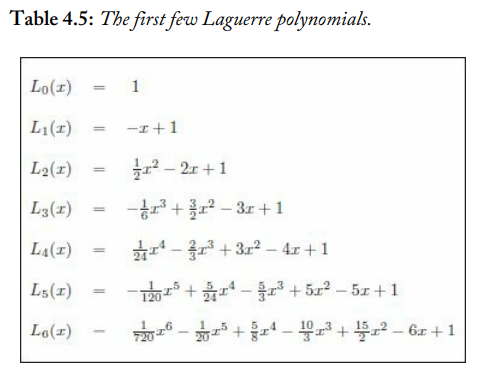
\includegraphics[width=0.5\textwidth]{Billeder/4.5.png} % Replace with your file
        \label{fig:subfig1}
    }
    %\hspace{0.05\textwidth} % Juster afstand mellem billeder
    % Second subfigure
    \subfloat[]{%
        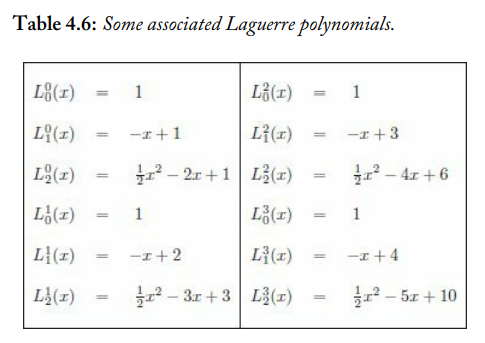
\includegraphics[width=0.5\textwidth]{Billeder/4.6.png}  % Replace with your file
        \label{fig:subfig2}
    }

\end{figure}

For hydrogen atomet gælder: 
\begin{align*}
    ψ_{nlm}\br{-\bar{r}} = \br{-1}^lψ_{nlm}\br{\bar{r}},
\end{align*}
hvis $l$ er lige er $ψ_{nlm}$ lige, og hvis $l$ er ulige er $ψ_{nlm}$ ulige. 

\n
\section{Impulsmoment}
Ved brug af den klassiske formel $\bar{L} = \bar{r} \times \bar{p}$, får vi kommutatorne for impulsmoment til: 
\begin{align*}
    \br[2]{L_x,L_y} = i\h L_z, \\
    \br[2]{L_y,L_z} = i\h L_x, \\
    \br[2]{L_z,L_x} = i\h L_y. \eq{4.99}
\end{align*}

Man kan ikke måle tilstande der er egenfnktioner til mere end en af disse,
men man kan finde en tilstand der er egenfunktion for $L^2 = L_x^2+L_y^2+L_z^2$ og en af de akse-specifikke. 
\begin{align*}
    L^2f=λf, \quad L_zf=μf. \eq{4.104}
\end{align*}

Vi laver en hæve sinke operator for impulsmomentet. 
\begin{align*}
    L_\pm = L_x \pm i L_y, \eq{4.105}
\end{align*}
hvor det gælder at 
\begin{align*}
    &\br[2]{L_z,L_\pm}=\pm\h L_\pm \eq{4.106}, \\
    &\br[2]{L^2,L_\pm} = 0 \eq{4.107}.
\end{align*}
Hvis $f$ er en egenfunktion for $L_z$ og $L^2$, med egenværdier. 
\begin{align*}
    &L^2(L_\pm f)=λ(L_\pm f), \eq{4.108} \\
    &L_z(L_\pm f) = (μ\pm \h)(L_\pm f). \eq{4.109}
\end{align*}

Hvis vi ser det som en trappe af trin hvor $L_\pm$ tager os et trin op eller ned, og man siger at trappen har $N$ trin, kan vi udregne egenværdierne til: 
\begin{align*}
    L^2 f_l^m = \h^2l(l+1)f_l^m ; \quad L_zf_l^m=\h mf_l^m. \eq{4.118}
\end{align*}
hvor $l=N/2$ og $m=-l,-l+1,...,l-1,l$. 

Vi kan udtrykke $L_x$ og $L_y$ ud fra $L_\pm$: 
\begin{align*}
    L_x &= \frac{L_++L_-}{2} \\
    L_y &= \frac{L_+-L_-}{2i}
\end{align*} 

Fra forlæsninger vedd vi: 
\begin{align*}
    L_\pm f_l^m = \h \sqrt{l(l+1)-m(m\pm 1)} f_l^{m\pm 1} \\
    \hv[f_l^m]{f_{l'}^{m'}} = δ_{l,l'}δ_{m,m'}
\end{align*}

Sammensætning med hydrogen: 
\begin{align*}
    f_l^m = Y_l^m \\
    \br[2]{H,L^2} = 0, \quad \br[2]{H,L_z} = 0, \quad \br[2]{L^2,L_z} = 0 \\
    \hv[ψ_{n,l,m}]{ψ_{n',l',m'}} = δ_{n,n'}δ_{l,l'}δ_{m,m'}
\end{align*}

\subsection{Matrixrepresentation}
Når man laver en operator som matrixrepræsentation i forhold til en basis af bølgefunktioner, får man hver indgang som: 
\begin{align*}
    \hv[ψ_{n,m,l}]{\hat{Q}ψ_{n',l',m'}}
\end{align*}
For eksempel for $n=2, l=1$: 

\begin{align*}
    [Q] = \begin{bmatrix}
        \hv[ψ_{2,1,-1}]{\hat{Q}ψ_{2,1,-1}} & \hv[ψ_{2,1,-1}]{\hat{Q}ψ_{2,1,0}} & \hv[ψ_{2,1,-1}]{\hat{Q}ψ_{2,1,1}} \\
        \hv[ψ_{2,1,0}]{\hat{Q}ψ_{2,1,-1}} & \hv[ψ_{2,1,0}]{\hat{Q}ψ_{2,1,0}} & \hv[ψ_{2,1,0}]{\hat{Q}ψ_{2,1,1}} \\
        \hv[ψ_{2,1,1}]{\hat{Q}ψ_{2,1,-1}} & \hv[ψ_{2,1,1}]{\hat{Q}ψ_{2,1,0}} & \hv[ψ_{2,1,1}]{\hat{Q}ψ_{2,1,1}}
    \end{bmatrix}
\end{align*}

Hvis man skriver bølgefunktionen op på matrixform, gøres det som enheds vektorer ud fra basen:
Dette gør det let at regne indre produkter, da $\hv{\hat{Q}ψ_{n,l,m}}$ er matrixerne ganget sammen. 

\section{Spin}
For spin infører vi en operator $S$ som i klassisk mekanink ville være $S=Iω$, og reglerne følger impulsmoment. 
\begin{align*}
    &\br[2]{S_x,S_y} = i\h S_z, \quad \br[2]{S_y,S_z} = i\h S_x, \quad \br[2]{S_z,S_x} = i\h S_y \eq{4.134} \\
    &S^2 \hv{sm} = \h^2 s(s+1)\hv{sm}, \quad S_z\hv{sm}=\h m \hv{sm} \eq{4.135} \\
    &S_\pm \hv{sm} = \h \sqrt{s(s+1)-m(m\pm 1)}\hv{s(m\pm 1)} \eq{4.136} \\
\end{align*}
Her har vi $s = 0, \frac{1}{2}, 1, \frac{3}{2}, ...$ og $m=-s, -s+1,...,s$ (4.137).
Protoner, neutroner, elektroner, lqptoner og quarks har $s=\frac{1}{2}$, dette spin kan vi udtrykke ved en spinor; $\hv{\uparrow}$ el. $\hv{\downarrow}$.
Matrixrepresentationen for S-operatoren for spin-$\frac{1}{2}$ er $S=\frac{\h}{2}σ$, hvor: 
\begin{align*}
    σ_x = \mat{0 & 1 \\ 1 & 0}, \quad σ_y = \mat{0 & -i \\ i & 0}, \quad σ_z = \mat{1 & 0 \\ 0 & -1}. \eq{4.148}
\end{align*}
Dertil har vi: 
\begin{align*}
    &S^2 = \frac{3}{4}\h^2 \mat{1 & 0 \\ 0 & 1} \eq{4.143} \\
    &S_+ = \h \mat{0 & 1 \\ 0 & 0 }, \quad S_- = \h \mat{0 & 0 \\ 1 & 0}. \eq{4.146}
\end{align*}

\newpage
\chapter{To-Partikel systemer}
Da vi nu har to partikler beskriver vi bølgefunktionen som en funktion af hver af partiklernes position, og tiden. 
\begin{align*}
    Ψ(\bar{r}_1, \bar{r}_2, t), 
\end{align*}
med Hamiltonian:
\begin{align*}
    \hat{H} = -\frac{\h^2}{2m_1}\nabla_1^2-\frac{\h^2}{2m_2}\nabla_2^2+V(\bar{r}_1, \bar{r}_2, t) \eq{5.3}
\end{align*}

På samme måde kan bølgefunktionen normeres med: 
\begin{align*}
    \int \br[5]{Ψ(\bar{r_1},\bar{r_2},t)}^2 d^3\bar{r_1}d^3\bar{r_2} = 1, \eq{5.5}
\end{align*} 
og opskrives som: 
\begin{align*}
    Ψ(\bar{r_1},\bar{r_2},t) = ψ(\bar{r_1},\bar{r_2})e^{iEt/\h}. \eq{5.6}
\end{align*}

Hvis de to partikler ikke interegere, kan bølgefunktionen beskrives som et produkt af 1-partikels bølgefunktioner: 
\begin{align*}
    & V(\bar{r}_1, \bar{r}_2) = V(\bar{r}_1) + V(\bar{r}_2), \eq{5.8} \\
    \Rightarrow & Ψ(\bar{r}_1, \bar{r}_2, t) = Ψ_a(\bar{r}_1,t) Ψ_b(\bar{r}_2,t). \eq{5.11}
\end{align*}

Når vi har identiske partikler findes der to slags. 

Bosoner opfylder at $ψ(\bar{r}_1, \bar{r}_2) = ψ(\bar{r}_2,\bar{r}_1)$, 
og fermioner opfylder at 

$ψ(\bar{r}_1, \bar{r}_2) = -ψ(\bar{r}_2,\bar{r}_1)$. 
Derudover har bosoner altid et heltal spin, mens fermioner har $n/2$ spin. To fermioner kan ikke optage den samme tilstand. 

For at få en symmetrisk bælgefunktion, kan man bruge formlen: 
\begin{align*}
    Ψ^{sym}(\bar{r}_1, \bar{r}_2) = A[Ψ(\bar{r}_1, \bar{r}_2) \pm Ψ(\bar{r}_1, \bar{r}_2)]. \eq{5.17}
\end{align*}

For forskellige partikler kan man regne middelværdien af positionen som: 
\begin{align*}
    \br[3]{\br{x_1-x_2}^2} &= \br[3]{x_1^2}+\br[3]{x_2^2}-2\br[3]{x_1x_2} \eq{5.22} \\
    &= \br[3]{x^2}_a+\br[3]{x^2}_b-2\br[3]{x}_b\br[3]{x}_b. \eq{5.23}
\end{align*}

For 2 identiske partikler har vi: 
\begin{align*}
    \br[3]{\br{Δx}^2}_\pm = \br[3]{\br{Δx}^2}_d \mp 2 \br[5]{\br[3]{x}_{ab}}^2, \eq{5.26}
\end{align*}
hvor subskriptet $+$ er for bosoner og $-$ er for fermioner, og 
\begin{align*}
    \br[3]{x}_{ab} = \int x ψ_a(x)^*ψ_b(x)dx. \eq{5.24}
\end{align*}

\n
\section{Spin}
Partikler kan også have spin, som tillader at fermioner kan være i samme tilstand, hvis de ahr forskelligt spin. 
I bogen noteres spin som $χ$. 
\begin{align*}
    ψ(\bar{r})χ, \eq{5.27} \\
    ψ(\bar{r}_1, \bar{r}_2)χ(1,2). \eq{5.28}
\end{align*}

Spinoren skal også opfylde kravet om symetri og antisymetri: 
\begin{align*}
    ψ(\bar{r}_1, \bar{r}_2)χ(1,2) = - ψ(\bar{r}_2, \bar{r}_1)χ(2,1). \eq{5.29}
\end{align*}

Hvis man skal lave et antisymetrisk spin, for fermioner har vi: 
\begin{align*}
    Ψ^{sym}(\bar{r}_1, \bar{r}_2) = ψ(\bar{r}_1) ψ(\bar{r}_2)\cdot \frac{χ(1,2)-χ(2,1)}{\sqrt{2}}. 
\end{align*}


\setcounter{chapter}{6}
\chapter{Pertubertionsregning}
Når vi har en pertubertion $H'$ har vi: 
\begin{align*}
    H = H^0+λH' \eq{7.4}
\end{align*}

Til første orden giver det os: 
\begin{align*}
    H^0ψ_n^1 + H'ψ_n^1 = E_n^0ψ_n^1+E_n^1ψ_n^0, \eq{7.5}
\end{align*}
og til anden orden: 
\begin{align*}
    H^0ψ_n^2 + H'ψ_n^1 = E_n^0ψ_n^2+E_n^1ψ_n^1+E_n^2ψ_n^0. \eq{7.6}
\end{align*}

Dermed får vi første orden energiforskydningen til: 
\begin{align*}
    E_n^1 = \hv[ψ_n^0]{H'ψ_n^0}. \eq{7.9}
\end{align*}

De tilsvarende bølgefunktioner kan findes ved: 
\begin{align*}
    ψ_n^1 = \sum_{m\neq n} \frac{\hv[ψ_m^0]{H'ψ_n^0}}{E_n^0-E_m^0}ψ_m^0. \eq{7.13}
\end{align*}

\n
\section{5 Trins Perturbationsregning}
Hvis man har et degenereret kvantesystem, det vil sige at flere niveuer kan have den samme energi, kan man ikke bruge oversående. 
Man skal i stedet bruge matrixrepræsentation af $H'$. Man skal starte med at vælge en basis: 
\[\{f_1, f_2, f_3\}\]

Derefter regner man matrixrepræsentation for $H'$: 
\begin{align*}
    [H'] = \mat{
        \hv[f_1]{H'f_1} & \hv[f_1]{H'f_2} & \hv[f_1]{H'f_3} \\
        \hv[f_2]{H'f_1} & \hv[f_2]{H'f_2} & \hv[f_2]{H'f_3} \\
        \hv[f_3]{H'f_1} & \hv[f_3]{H'f_2} & \hv[f_3]{H'f_3} } \eq{7.40}
\end{align*}

For at finde energiskiftende, skal man finde egenværdierne $(e_n)$ til $[H']$, 
og bølgefunktion findes som den lineære kombination af egenvektoren $(v_n$ til hver af energiskiftende. 

\begin{align*}
    E_n^0 = \begin{cases}
        E_n^0+e_1 \\ 
        E_n^0+e_2 \\
        E_n^0+e_3
    \end{cases}
\end{align*}




\end{document} % ----------Dokumentet er nu slut! ------------